\section{Zielsetzung}
\label{sec:Zielsetzung}
Es soll die Suszeptibilität paramgnetischer Stoffe bestimmt werden. Dies wird durch eine Brückenschaltung für
drei verschiedene seltene Erden realisiert.

\section{Theorie}
\label{sec:Theorie}
Die magnetische Flussdichte $\vec{B}$ und die magnetische Feldstärke $\vec{H}$ hängen in Materie durch die
Beziehung
\begin{equation}
    \vec{B} = \mu_{0}\vec{H}+\vec{M}
\end{equation}
ab. Dabei ist $\vec{M}$ die Magnetisierung und $\mu_{0}$ die magnetische Feldkonstante. $\vec{M}$ hängt von
$\vec{H}$ durch die Suszeptibilität $\chi$ durch
\begin{equation}
    \vec{M} = \mu_{0}\left(\chi+1\right)\vec{H}
\end{equation}
ab. $\chi$ ist dabei keineswegs eine Konstante, sondern hängt in komplizierter Weise von $\vec{H}$ und der
Temperatur $T$ ab. Allgemein tritt für alle Atome der Diamagnetismus auf, da er durch ein von außen angelegtes
Magnetfeld magnetische Momente im Atom induziert, so dass ein dem äußeren entgegengestztes Magnetfeld induziert
wird. In diesem Fall ist $\chi < 0$. Im Gegensatz dazu tritt der Paramagnetismus nur bei Atomen, Molekülen oder
Ionen auf, die keinen verschwindenden Gesamtdrehimpuls $\vec{J}$ haben. Er entsteht dadurch, dass sich die mit
dem Drehimpuls gekoppelten magnetischen Momente relativ zum äußeren Magnetfeld ausrichten. Da die magnetischen
Momente durchgängig durch die thermische Bewegung gestört werden, ist der Paramagnetismus temperaturabhängig.
Für den Diamagnetismus trifft dies nicht zu. Der Gesamtdrehimpuls setzt sich aus dem Bahndrehimpuls $\vec{L}$
und dem Spin $\vec{S}$ durch
\begin{equation*}
    \vec{J} = \vec{L} + \vec{S}
\end{equation*}
zusammen. Die magnetischen Momente zum Drehimpuls und Spin ergeben sich zu
\begin{equation*}
    \vec{\mu}_{\symup{L}} = -\frac{\mu_{\symup{B}}}{\hbar} \vec{L}
\end{equation*}
und
\begin{equation*}
    \vec{\mu_{\symup{S}}} =  -g_{\symup{S}}\frac{\mu_{\symup{B}}}{\hbar}\vec{S}\,.
\end{equation*}
$\hbar$ ist dabei das reduzierte Plancksche Wirkungsquantum, $\mu_{\symup{B}}=\frac{e_{0}\hbar}{2m_{0}}$ das
Bohrsche Magneton und $g_{\symup{S}}$ das gyromagnetische Verhältnis des freien Elektrons.
\begin{figure}
    \centering
    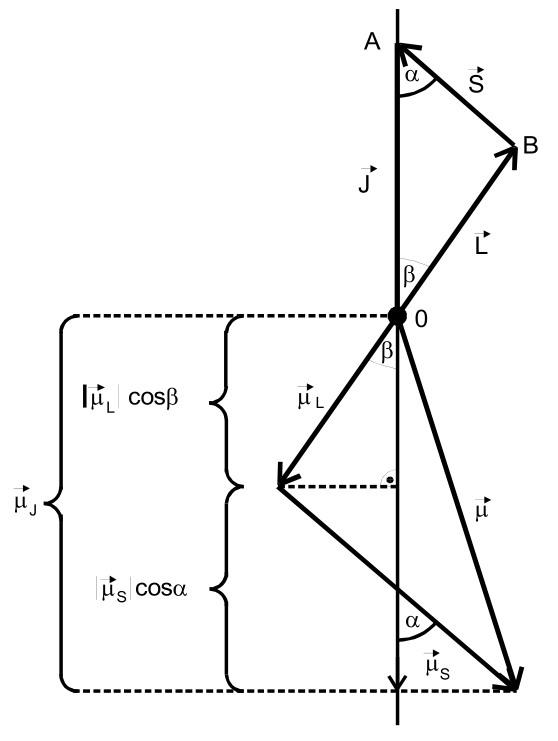
\includegraphics[width=0.4\textwidth]{bilder/vektordiagramm.png}
    \caption{Vektordiagramm der Drehimpulsvektoren und den magnetischen Momenten \cite{sample}.}
    \label{fig:vektordiagramm}
\end{figure}
Aus den geometrischen Zusammenhänge aus \autoref{fig:vektordiagramm} ergibt sich
\begin{equation*}
    |\vec{\mu_{\symup{J}}}| = |\vec{\mu_{\symup{S}}}|\cos{\alpha}| + |\vec{\mu_{\symup{L}}}|\cos{\beta}
\end{equation*}
Weiterhin gelten für $|\vec{\mu_{\symup{L}}}|$ und $|\vec{\mu_{\symup{S}}}|$
\begin{align*}
    |\vec{\mu_{\symup{L}}}| &= \mu_{\symup{B}}\sqrt{L\left(L+1\right)} \\
    |\vec{\mu_{\symup{S}}}| &= g_{\symup{S}}\mu_{\symup{B}}\sqrt{S\left(S+1\right)}\,.
\end{align*}
Mit Hilfe des durch
\begin{equation*}
    g_{\symup{J}} = \frac{3J\left(J+1\right) + S\left(S+1\right)- L\left(L+1\right)}{2J\left(J+1\right)}
\end{equation*}
definierten Lande-Faktors ergibt sich dann
\begin{equation*}
    |\vec{\mu_{\symup{J}}}| \approx \mu_{\symup{B}}g_{\symup{J}}\sqrt{J\left(J+1\right)}\,.
\end{equation*}
Daraus ergibt sich dann die potentielle Energie der Ausrichtung mit der Ausrichtungsquantenzahl $m$ zu
\begin{equation}
    E_{\symup{m}} = \mu_{\symup{B}}g_{\symup{J}}m\,.
\end{equation}
Anschließend spalten sich die Energieniveaus durch den Zeeman-Effekt auf. Um nun die Magnetisierung zu bestimmen
wird ein mittleres magnetisches Moment bestimmt, dass sich mit Hilfe der Brillouin-Funktion bestimmen lässt.
Die magnetischen Momente sind nach der Boltzmann-Verteilung verteilt. Da sich im Allgemeinen eine tranzendente
Gleichung ergibt, wird eine Näherung für hohe Temperaturen bzw. Raumtemperatur und schwache Felder benutzt,
so dass sich die Magnetisierung zu
\begin{equation*}
    M = \frac{1}{3}\mu_{0}Ng^{2}_{\symup{J}}\mu^2_{\symup{B}}\frac{J\left(J+1\right)B}{kT}
\end{equation*}
und daraus die Suszeptibilität zu
\begin{equation}
    \label{eqn:chi}
    \chi = \frac{1}{3}\mu_{0}Ng^{2}_{\symup{J}}\mu^2_{\symup{B}}\frac{J\left(J+1\right)}{kT}\,.
\end{equation}
Es ergibt sich die aus dem Curieschen Gesetz bekannte $\frac{1}{T}$-Abhängigkeit des Paramagnetismus.

\subsection{Suszeptibilität seltener Erden}
\label{sec:selteneErden}
Da seltene Erden einen starken Paramagnetismus aufweisen, müssen die Elektronenhüllen große Drehimpulse aufweisen.
Dies lässt sich durch die $4f$-Elektronen erklären, die in der $6s$-Schale liegen und erst ab Ordnungszahlen größer
gleich $58$ auftreten. Der Gesamtdrehimpuls der $6s$-Schale lässt sich mit Hilfe der Hundschen Regeln bestimmen.
Wenn die Schale weniger als die Hälfte gefüllt ist, bestimmt sich der Gesamtdrehimpuls zu $\vec{J}=\vec{L}-\vec{S}$
und wenn die Schale mehr als die Hälfte gefüllt ist, bestimmt sich der Gesamtdrehimpuls zu
$\vec{J}=\vec{L}+\vec{S}$. Dabei gilt für $\vec{L}$ und $\vec{S}$
\begin{align*}
    \vec{L} = \sum_{\symup{i}} \vec{l_{\symup{i}}}\\
    \vec{S} = \sum_{\symup{i}} \vec{s_{\symup{i}}}\,.
\end{align*}

\subsection{Messapparatur zur Bestimmung der Suszeptibilität}
\label{sec:Messapparatur}
Um ein Magnetfeld zu erzeugen wird eine lange Spule verwendet, da in ihrem Inneren das Magnetfeld annähernd homogen
ist. Für das Induktivität $L$ einer langen Spule gilt
\begin{equation*}
    L = \mu_{0}\frac{n^2}{l}F\,.
\end{equation*}
Dabei sind $n$ die Anzahl der Windungen $l$ die Länge der Spule und $F$ der Querschnitt der Spule. Um den Umstand
mit ein zu beziehen, dass die Probe die Spule nicht ganz ausfüllt, kann die Formel zu
\begin{equation}
    L_{\symup{M}} = \mu_{0}\frac{n^{2}F}{I}+\chi\mu_{0}\frac{n^{2}Q}{I}
\end{equation}
bestimmt werden, wobei $Q$ der Querschnitt der Spule ist. Da die Induktivitäten der gefüllten Spule und der im
Vakuum nur sehr gering ist, wird eine hohe Messauflösung benötigt. Zur Messung werden deshalb zwei
möglichst identische Spulen verwendet. In die eine Spule wird die Messprobe eingeführt und die andere wird leer
gelassen. Mit Hilfe einer Brückenschaltung lässt sich nun die Suszeptibilität über zwei Methoden bestimmen.
Der Schaltplan der verwendeten Brückenschaltung ist in \autoref{fig:bruecke} angegeben.
\begin{figure}
    \centering
    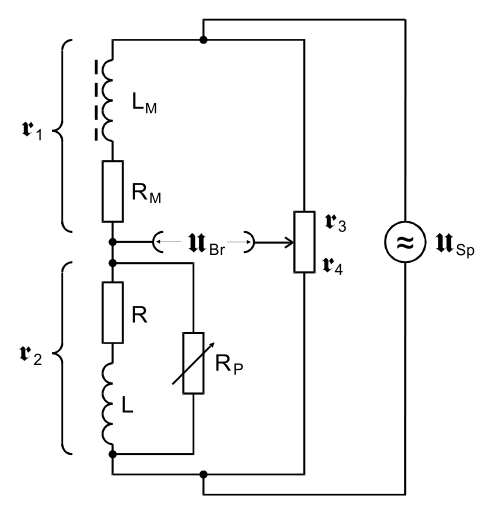
\includegraphics[width=0.4\textwidth]{bilder/bruecke.png}
    \caption{Brückenschaltung zweier Spulen zur Bestimmung der Suszeptibilität \cite{sample}.}
    \label{fig:bruecke}
\end{figure}
Bei der ersten Methode wird nach Abgleichen der Brücke die Spannung $U_{\symup{Br}}$ gemessen, wenn die Probe
eingeführt wird. Bei der zweiten Methode wird die Brücke wieder zuerst abgeglichen und nach Einführen der Probe
erneut abgeglichen. Aus der Änderung der Abgleichelemente kann dann die Suszeptibilität bestimmt werden.
Für die erste Methode bestimmt sich $\chi$ unter Verwendung der Knoten- und Maschenregel, dem Umstand,
dass $\symup{\Delta}L << L$ gilt und der Annahme, dass hinreichen hohe Messfrequenzen verwendet werden, zu
\begin{equation}
    \label{eqn:chiSp}
    \chi = 4\frac{F}{Q}\frac{U_{\symup{Br}}}{U_{\symup{Sp}}}\,.
\end{equation}
Für die zweite Methode wird $\chi$ unter Verwendung der Abgleichbedingung $r_{1}R_{4}=r_{2}R_{3}$ für eine kleine
Abweichung $\symup{\Delta}R$ und der Annäherung $\symup{\Delta}L << L$ zu
\begin{equation}
    \label{eqn:chiWd}
    \chi = 2 \frac{\symup{\Delta}R}{R_{3}}\frac{F}{Q}
\end{equation}
bestimmt.

\subsection{Verfahren zur Unterdrückung der Störspannung}
\label{sec:stoer}
Die Messung der Brückenspannung stellt sich als schwierig dar, da Störspannungen an den Ausgangsklemmen die
Brückenspannung überdecken können. Da es sich um monofrequente Signalspannungen handelt, lässt sich dieses
Problem mit Hilfe eines Selektivverstärkers eleiminieren. Dabei ist die Filterkurve eines Selektivverstärkers
eine Glockenkurve, wie in \autoref{fig:Filterkurve} abgebildet.
\begin{figure}
    \centering
    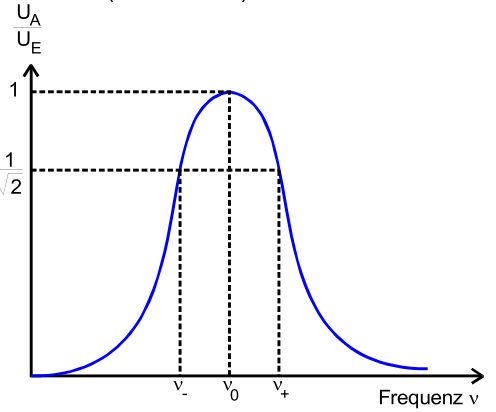
\includegraphics[width=0.4\textwidth]{bilder/filterkurve.png}
    \caption{Fiterkurve eines Selektrivverstärkers \cite{sample}.}
    \label{fig:Filterkurve}
\end{figure}
Die Filterkurve beschreibt die Abhängigkeit des Quotienten aus Ausgangs- und Eingangsspannung
$\frac{U_{\symup{A}}}{U_{\symup{B}}}$ zur Frequenz $\nu$. Dabei gilt die Breite der Filterkurve ist proportional
zur Spannungsunterdrückung. Dieser Zusammenhang lässt sich durch die Güte $Q$ eines Selektivverstärkers
durch
\begin{equation}
    \label{eqn:Guete}
    Q = \frac{\nu_{0}}{\nu_{+}-\nu_{-}}
\end{equation}
ausdrücken. Hier sind $\nu_{\pm}$ die Frequenzen bei denen die Filterkurve den Werte $\frac{1}{\sqrt{2}}$ erreicht
haben.